% \pdfminorversion=4
\documentclass{beamer}
\usepackage[utf8]{inputenc}
\usepackage{indentfirst}
\usepackage{enumitem}
\usepackage{datetime2}
\usepackage{acronym}
% options (https://tex.stackexchange.com/questions/25520/how-can-i-use-the-latex-acronym-package-and-optionally-create-an-acronym-list-i):
% printonlyused: Only list used acronyms
% withpage: In printonlyused-mode show the page number where each acronym was first used.
% nolist: The option nolist stands for “don’t write the list of acronyms”.
% dua: The option dua stands for “don’t use acronyms”. It leads to a redefinition of \ac and \acp, making the full name appear all the time and suppressing all acronyms but the explicity requested by \acf or \acfp.

\makeatletter
\AtBeginDocument{%
  \renewcommand*{\AC@hyperlink}[2]{%
    \begingroup
      \hypersetup{hidelinks}%
      \hyperlink{#1}{#2}%
    \endgroup
  }%
}
\makeatother

\usepackage{algorithm}
\usepackage{algpseudocode}

\usepackage{textcomp}
\usepackage[T1]{fontenc}
\usepackage{multirow,bigdelim}
\usepackage{float}
\usepackage[caption = false]{subfig}
\usepackage{longtable}
\usepackage{listings}
\usepackage{mathtools}
\DeclareMathOperator{\tr}{Tr}
\usepackage{commath}
\usepackage{slashed}
\usepackage{bbold}
\usepackage{xcolor}
\usepackage{physics}
\newcommand{\lambdabar}{{\mkern0.75mu\mathchar '26\mkern -9.75mu\lambda}}
\usepackage[right=4cm,left=2cm,top=3cm,bottom=3.0cm, marginparwidth=2.7cm, marginparsep=3mm]{geometry}
\usepackage{mdframed}


\usepackage{amsmath}
\usepackage{amsfonts}
\usepackage{amssymb}

\numberwithin{equation}{section}
\usepackage{graphicx}

\usepackage[colorinlistoftodos]{todonotes}
\PassOptionsToPackage{hyphens}{url}
\usepackage[colorlinks=true, allcolors=blue]{hyperref}
\hypersetup{breaklinks=true}

% \urlstyle{same}
\usepackage{siunitx}
\sisetup{separate-uncertainty=true}
% \DeclareSIUnit\parsec{pc}
\usepackage{cancel}
\usepackage{mathrsfs}
\usepackage{marginnote}
\renewcommand*{\marginnotevadjust}{-0.3cm}
\renewcommand*{\marginfont}{\scriptsize}
% \usepackage{fancybox}

\usepackage{footnotebackref}

\usepackage[sc]{mathpazo}
\linespread{1.05}         % Palladio needs more leading (space between lines)
\usepackage[T1]{fontenc}

\newcommand\mybox[1]{%
  \fbox{\begin{minipage}{0.9\textwidth}#1\end{minipage}}}

\newcommand{\const}{\mathrm{const}}

\usepackage[section]{placeins}

\usepackage{tikz}
\usetikzlibrary{shapes,arrows,shadows}


\newcommand{\boxalign}[2][0.986\textwidth]{
  \par\noindent\tikzstyle{mybox} = [draw=black,inner sep=6pt]
  \begin{center}\begin{tikzpicture}
   \node [mybox] (box){%
    \begin{minipage}{#1}{\vspace{-5mm}#2}\end{minipage}
   };
\end{tikzpicture}\end{center}}


\pagestyle{plain}

\author{Jacopo Tissino}

\allowdisplaybreaks
\usetheme{Rochester}
% \usepackage[scaled]{helvet} % ss

\usepackage[
backend=biber,
style=authoryear,
sorting=nyt,
urldate=iso8601,
url=false,
isbn=false,
doi=false
]{biblatex}

\title{Machine Learning Gravitational Waveforms for Binary Neutron Star mergers}
\author{Jacopo Tissino}
\date{2021-09-10}

\addbibresource{../notes/Masters_thesis.bib}


\begin{document}

\frame{\titlepage}

\begin{frame}
    \frametitle{Amplitudes}
    \begin{figure}[ht]
    \centering
    \includegraphics[width=\textwidth]{figures/native_amplitudes}
    \label{fig:native_amplitudes}
    \end{figure}
\end{frame}

\begin{frame}
    \frametitle{Phases}
    \begin{figure}[ht]
    \centering
    \includegraphics[width=\textwidth]{figures/native_phases}
    \label{fig:native_phases}
    \end{figure}
\end{frame}

\begin{frame}
    \frametitle{MLGW\_BNS structure: training dataset generation}
    \begin{itemize}
    \item Greedy adaptive downsampling fit;
    \item EOB waveform generation and downsampling;
    \item residuals from PN waveforms: \(\Delta A = \log (A _{\text{EOB}}/ A _{\text{PN}})\) and \(\Delta \Phi = \Phi _{\text{EOB}} - \Phi _{\text{PN}}\);
    \item PCA on the combined, downsampled, rescaled residuals;
    \item a NN learns the map \(\theta \to PC_i \lambda_i^{\alpha}\);
    \item the hyperparameters of the NN and \(\alpha \) are optimized case-by-case.
    \end{itemize}
\end{frame}

\begin{frame}
    \frametitle{Residuals: amplitude}
    \begin{figure}[ht]
    \centering
    \includegraphics[width=\textwidth]{figures/amp_residuals}
    \label{fig:amp_residuals}
    \end{figure}
\end{frame}

\begin{frame}
    \frametitle{Residuals: phase}
    \begin{figure}[ht]
    \centering
    \includegraphics[width=\textwidth]{figures/phase_residuals}
    \label{fig:phase_residuals}
    \end{figure}
\end{frame}

\begin{frame}
    \frametitle{PCA mismatches}
    \begin{figure}[ht]
    \centering
    \includegraphics[width=.9\textwidth]{figures/mismatches_PCA}
    \label{fig:mismatches_PCA}
    \end{figure}
\end{frame}

\begin{frame}
    \frametitle{Hyperparameter optimization}
    \begin{figure}[ht]
    \centering
    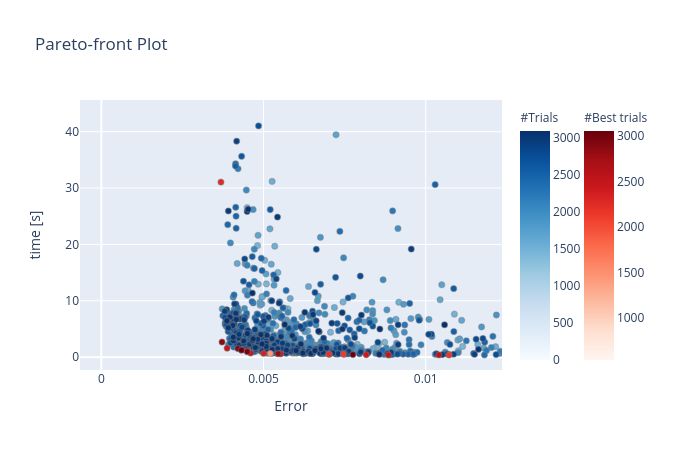
\includegraphics[width=\textwidth]{figures/pareto-front-nonspinning}
    \label{fig:pareto-front-nonspinning}
    \end{figure}
\end{frame}

\begin{frame}
    \frametitle{Fidelity: nonspinning case}
    \begin{figure}[ht]
    \centering
    \includegraphics[width=\textwidth]{figures/mismatches_nonspinning}
    \label{fig:mismatches_nonspinning}
    \end{figure}
\end{frame}

\begin{frame}
    \frametitle{Fidelity: spinning case}
    \begin{figure}[ht]
    \centering
    \includegraphics[width=\textwidth]{figures/mismatches_spinning}
    \end{figure}
\end{frame}

\begin{frame}
    \frametitle{Amplitude reconstruction residuals}
    \begin{figure}[ht]
    \centering
    \includegraphics[width=\textwidth]{figures/recon-amp-residuals}
    \label{fig:recon-amp-residuals}
    \end{figure}
\end{frame}

\begin{frame}
    \frametitle{Phase reconstruction residuals}
    \begin{figure}[ht]
    \centering
    \includegraphics[width=\textwidth]{figures/recon-phase-residuals}
    \label{fig:recon-phase-residuals}
    \end{figure}
\end{frame}


\begin{frame}
    \frametitle{Evaluation time: \(f_0 = \SI{20}{Hz}\)}
    
    \begin{figure}[ht]
    \centering
    \includegraphics[width=\textwidth]{figures/evaluation_time_by_fsize}
    \label{fig:evaluation_time_by_fsize}
    \end{figure}
\end{frame}

\begin{frame}
    \frametitle{Evaluation time: \(f_0 = \SI{20}{Hz}\)}
    
    \begin{figure}[ht]
    \centering
    \includegraphics[width=\textwidth]{figures/overhead_evaluation}
    \label{fig:overhead_evaluation}
    \end{figure}
\end{frame}

\begin{frame}
    \frametitle{Evaluation time: \(f_0 = \SI{20}{Hz}\)}
    
    \begin{figure}[ht]
    \centering
    \includegraphics[width=\textwidth]{figures/teobresumspa_speedup}
    \label{fig:teobresumspa_speedup}
    \end{figure}
\end{frame}

\begin{frame}
    \frametitle{Evaluation time: \(f_0 = \SI{10}{Hz}\)}    
    \begin{figure}[ht]
    \centering
    \includegraphics[width=\textwidth]{figures/evaluation_time_by_fsize_10hz}
    \label{fig:evaluation_time_by_fsize}
    \end{figure}
\end{frame}

\begin{frame}
    \frametitle{Evaluation time: \(f_0 = \SI{10}{Hz}\)}
    
    \begin{figure}[ht]
    \centering
    \includegraphics[width=\textwidth]{figures/overhead_evaluation_10hz}
    \label{fig:overhead_evaluation}
    \end{figure}
\end{frame}

\begin{frame}
    \frametitle{Evaluation time: \(f_0 = \SI{10}{Hz}\)}
    
    \begin{figure}[ht]
    \centering
    \includegraphics[width=\textwidth]{figures/teobresumspa_speedup_10hz}
    \label{fig:teobresumspa_speedup}
    \end{figure}
\end{frame}

\begin{frame}
    \frametitle{Profiling the evaluation: \(\num{e4}\) interpolation points}
    \begin{figure}[ht]
    \centering
    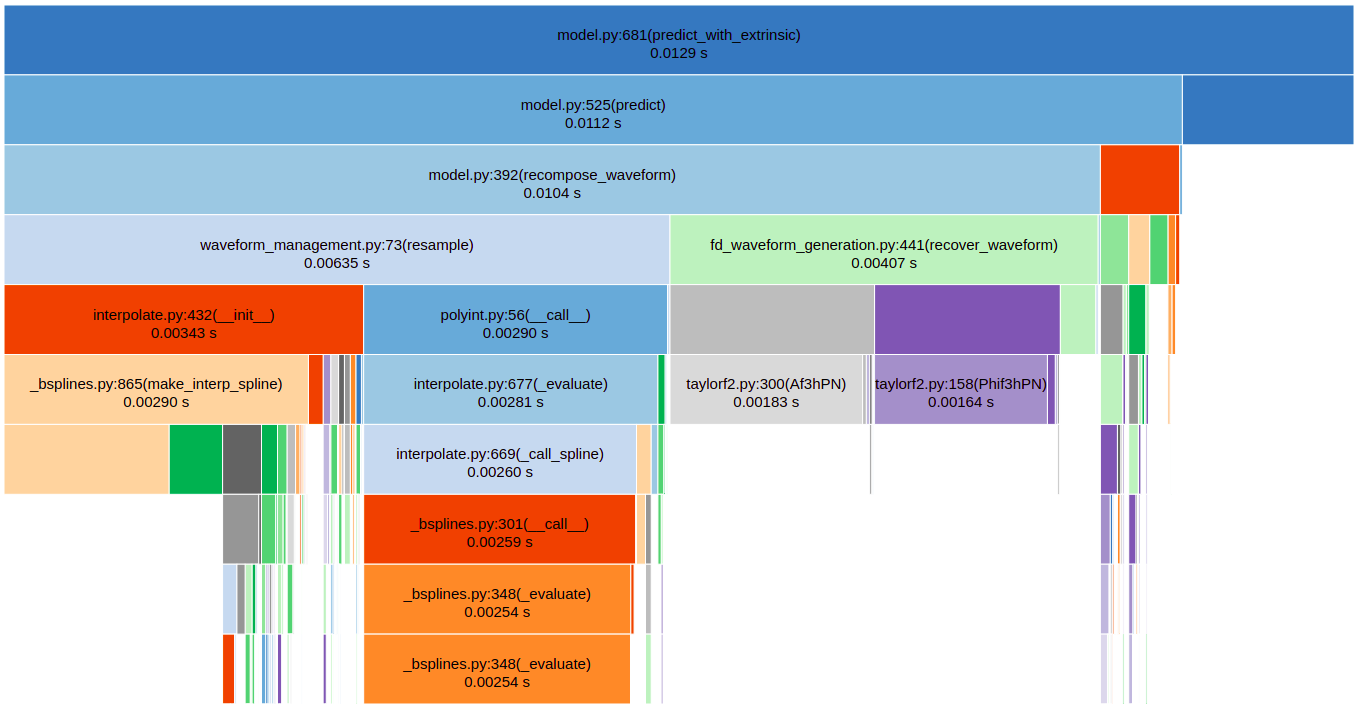
\includegraphics[width=\textwidth]{figures/predict_profile_fast}
    \label{fig:predict_profile_fast}
    \end{figure}
\end{frame}

\begin{frame}
    \frametitle{Profiling the evaluation: \(\num{e6}\) interpolation points}
    \begin{figure}[ht]
    \centering
    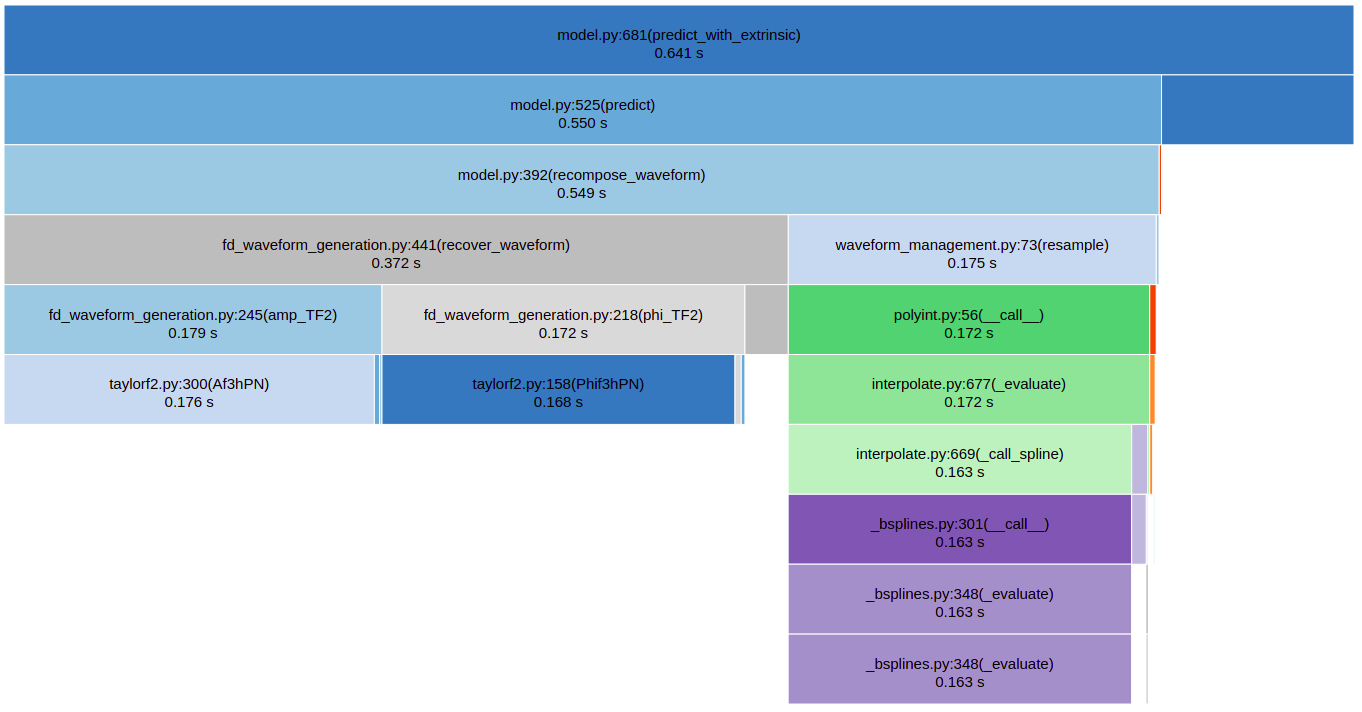
\includegraphics[width=\textwidth]{figures/predict_profile_slow}
    \label{fig:predict_profile_slow}
    \end{figure}
\end{frame}

\begin{frame}
    \frametitle{Fourier transform issues}
    
    \begin{figure}[ht]
    \centering
    \includegraphics[width=\textwidth]{figures/FFT-noise-wide}
    \label{fig:fft-noise-wide}
    \end{figure}
\end{frame}

\begin{frame}
    \frametitle{Fourier transform issues}
    
    \begin{figure}[ht]
    \centering
    \includegraphics[width=\textwidth]{figures/FFT-noise-highf}
    \label{fig:fft-noise-highf}
    \end{figure}
\end{frame}

\begin{frame}
    \frametitle{Fourier transform issues}
    
    \begin{figure}[ht]
    \centering
    \includegraphics[width=\textwidth]{figures/FFT-noise-lowf}
    \label{fig:fft-noise-lowf}
    \end{figure}
\end{frame}



% \begin{frame}
%     \frametitle{}
    
% \end{frame}


% \begin{frame}
%     \frametitle{Bibliography}
%     \printbibliography
% \end{frame}


\end{document}
